\documentclass[a4paper]{article}   % On declare le type du document : article, book, beamer (pour une presentation)... %  a4paper car c'est le format standard du papier en Europe.

%%%% Packages

\usepackage{lmodern}
\usepackage[french]{babel}  		% on écrit en français
\usepackage[utf8x]{inputenc} 		% pour utiliser toutes les touches du clavier
\usepackage[T1]{fontenc}  		% pour utiliser toutes les touches du clavier
\usepackage{pifont}
\usepackage[dvips]{graphicx}  		%Pour Compiler en LaTeX    %%%%%%%%
\usepackage{graphics}        		% Pour Compiler en LaTeX    %%%%%%%% ATTENTION!!!! pour sortir du TeXgraph en pdf il faut le package graphicx dans le préambule et includegraphics{*.pdf} dans le dodument. Mais cela fait foirer la compilation LaTeX.
\usepackage[dvips]{graphicx}        	%pour le pdf
\usepackage{multirow}
\usepackage{epsfig}			% Pour importer une image
\usepackage{variations}  			% Tableaux de variations

\usepackage{minibox}
\usepackage{marvosym}
%\usepackage{hyperref}
\usepackage{enumerate}
\usepackage{wrapfig}
\usepackage{multicol}
\usepackage{framed}
\usepackage{verbatim}
\usepackage[mathcal,mathscr]{eucal} 
\usepackage{eufrak}
\usepackage[np]{numprint}
\usepackage{tabularx}
\usepackage{fancybox}
\usepackage{amsmath,amsfonts, amssymb}  % Des pack de l'AMS tres utiles en math
\usepackage{lmodern}           		% Ameliore la mise en page des textes francais 
\usepackage{enumerate}         		% Pour faire des listes numerotees.
\usepackage[colorlinks=true,urlcolor=blue]{hyperref} % Liens hyper-textes ...% ...utiles pour un document en ligne,
\usepackage{color}    	% Pour écrire en couleur:  {\color{red} bla} ou {\color[rgb]{0,0,1} bla} [red, green, blue]		
\usepackage{amsthm}
\usepackage[a4paper]{geometry}    	% pour aggrandir ou diminuer les marges.                           
\geometry{a4paper,left=2cm,right=2cm,top=1cm,bottom=1.5cm}

\renewcommand\thesection {\Roman{section}-}	% pour avoir les sections en grec
\renewcommand{\(}{\left(}
\renewcommand{\)}{\right)}
\newcommand{\e}{\,\text{e}\,} 
\newcommand{\limit}[2]{\lim\limits_{#1 \to #2}}

%%%

\definecolor{CouleurA}{rgb}{0, 0, 0} %noir
\definecolor{CouleurB}{rgb}{0.77751, 0.2511, 0.13799}
\definecolor{CouleurC}{rgb}{0.85895, 0.93161, 0.10727}
\newenvironment{TraitV}[3][CouleurA]{%
% #1 couleur du trait (par défaut CouleurA)
% #2 largeur du trait
% #3 distance entre le trait et le texte
\def\FrameCommand{{\color{#1}\vrule width #2}
\hspace{#3}}%
\MakeFramed {\advance\hsize-\width}}%
{\endMakeFramed}

%%%

\renewcommand{\theenumi}{\textbf{\arabic{enumi}}}
\renewcommand{\labelenumi}{\textbf{\theenumi.}}
\renewcommand{\theenumii}{\textbf{\alph{enumii}}}
\renewcommand{\labelenumii}{\textbf{\theenumii.}}

%%%% Théorèmes Français numérotés

\newtheorem{de}{Définition}		% Syntaxe : \begin{de} la li la la \end{de} .
\newtheorem{theom}{Théorème}
\newtheorem{propo}{Propriété}
\newtheorem{que}{Question}
\newtheorem{ques}{~}
\newenvironment{qu}{\begin{ques}--} {\end{ques}}
\newtheorem{rmq}{Remarque}
\newtheorem{exm}{Exemple}
\newtheorem{exoit}{Exercice}
\newenvironment{exo}   {\begin{exoit} \normalfont}
               {\end{exoit} \medskip}			% Les exercices ne seront pas en italique.
\newtheorem{EXO}{\large EXERCICE }
\newenvironment{EX}   { \setcounter{ques}{0} \begin{EXO} \hrulefill ~\vspace{0.3cm}

\normalfont}    {\end{EXO} \medskip}			
\newenvironment{ex}   {\begin{exm} \normalfont}
               {\end{exm} \medskip}			% Les exemples ne seront pas en italique.
\newtheorem*{demo*}{Démonstration}		
\newenvironment{dem}   {\begin{demo*}\normalfont : \begin{TraitV}{1.5pt}{10pt}} 
               {\end{TraitV}\end{demo*}\medskip}	
\newenvironment{thm}{\begin{Sbox}\begin{minipage}{0.9\linewidth}\begin{theom} ---}		% les théorèmes seront encadrés.
{\end{theom}\end{minipage}\end{Sbox}\begin{center}\fbox{\TheSbox}\end{center}}
\newenvironment{prop}{\begin{Sbox}\begin{minipage}{0.9\linewidth}\begin{propo} ---}		% les propriétés seront encadrées.
{\end{propo}\end{minipage}\end{Sbox}\begin{center}\fbox{\TheSbox}\end{center}}


%%%%  Nouveaux opérateurs.

\DeclareMathOperator{\diver}{\operatorname{div}}
\DeclareMathOperator{\rot}{\operatorname{rot}}
\DeclareMathOperator{\supp}{\operatorname{Supp}}
\DeclareMathOperator{\conv}{\operatorname{Conv}}

%%%% Raccourcis 
% Par exemple, quand on tapera \R, le code comprendra \mathbb R  qui utilise la bonne police pour écrire l'ensemble des reels.

\newcommand{\R}{ ${\mathbb R} ~$}
\newcommand{\C}{ ${\mathbb C} ~$}
\newcommand{\Z}{ ${\mathbb Z} ~$}
\newcommand{\N}{ ${\mathbb N} ~$}
\newcommand{\Nn}{ ${\mathbb N^*} ~$}
\newcommand{\divpart}[1]{{\displaystyle \frac{\partial #1}{\partial t}}}
\newcommand{\divdroite}[1]{{\displaystyle \frac{d #1}{ dt}}}
\newcommand{\ep}{{\varepsilon}}
\newcommand{\ddt}{{\frac{d}{dt}}}
\newcommand{\dronde}{ {\frac{\partial}{\partial t} }}
\newcommand{\cf}{$\mathcal{C}~$} 	%courbe Cf
\newcommand{\df}{$\mathcal{D}~$} 	%ensemble de définition Df
\newcommand{\ie}{\leqslant ~}  		% pr < ou= et > ou=
\newcommand{\se}{\geqslant~} 		% pr < ou= et > ou=
\newcommand{\ri}{$\left(O;\vec{i};\vec{j}\right)$}
\newcommand{\ru}{$\left(O;\vec{u};\vec{v}\right)$} 	% repères
\newcommand{\f}{\dfrac} 	% =\dfrac = \frac avec displaystyle
\def\v{\overrightarrow}	% vecteur : syntaxe : $\v{AB}$
\newcommand{\al}{\quad \Rightarrow \quad}	% implication
\newcommand{\ssi}{\quad \Leftrightarrow \quad}	% équivalence
\newcommand{\ass}{\mapsto~}		% flèche de "fonction qui a x associe..."
\newcommand{\x}{\times} %pour le symbole x

% \lim\limits_{n \to +\infty} v_n=+\infty  ; limite
% Type de document - classe - date [à faire avec mise en page]

		% Titre chapitre
%\def\dev{DS de mathématiques n°}
%\def\dev{DM de Mathématiques n°}
%\def\dev{Correction des Exercices - Fonctions Trinômes}
%\def\dev{Correction du DM n°}
%\def\dev{ Test de math}
%def\dev{ Autre }
%\def\numero{10}                         % Numéro du devoir
%\def\cl{{\Large \bf{2nde}}} 	% Classe
%\def\cl{{\large \bf{Term STMG}}}
\def\cl{{\large \bf{1èreG1}}}
\def\jour{le 07/10/2020}                  % Date

%%%%%%%%%%%%%%%%%%%%%%%%%%%%%%%%%%%%%%%%%%%%%%%%
%%%%%%%%%%%%%%%%%%%%%%%%%%%%%%%%%%%%%%%%%%%%%%%%
%%%%%%%%%%%%%%%%%%%%%%%%%%%%%%%%%%%%%%%%%%%%%%%%

\begin{document}			% Le document commence ici.

\newpage 

\def\dev{\Large Polynômes du second degré}
\noindent\begin{minipage}{.20\linewidth}\begin{center}                  
\noindent \emph{Lycée Paul Lapie - Courbevoie}
\end{center}\end{minipage}
\begin{minipage}{1.5\linewidth}\begin{center}	
\noindent \cl\\ Chapitre 1
\end{center}\end{minipage}

\begin{center}\shadowbox{ \Large Planche n°1  : \dev } 	
\end{center}
{\large{

\begin{EX} Mettre les polynômes sous forme canonique :

\begin{enumerate}
\renewcommand{\tabularxcolumn}[1]{b{#1}}
\begin{tabularx}{\linewidth}{XX}	
\item $f(x)=-4x^2 +24x+11$& 
\item $g(x)=3x^2+9x+1$ \\
\item $h(x)=x^2-5x$ &
\item $k(x)=-2x^2-8x+3$ \\
\end{tabularx}
\end{enumerate}


\end{EX}

\begin{EX} Résoudre les équations suivantes :
\begin{enumerate}
\renewcommand{\tabularxcolumn}[1]{b{#1}}
\begin{tabularx}{\linewidth}{XX}	
\item $x^2-3x+1=0$&
\item $2x^2+x+1=0$ \\
\item $0.3x^2-3x-7.5=0$&
\item $18x^2-12x+2=0$\\
\end{tabularx}
\end{enumerate}
\end{EX}

\begin{EX} Déterminer les racines éventuelles, et en déduire, si possible, une expression factorisée des trinômes suivants :
\begin{enumerate}
\renewcommand{\tabularxcolumn}[1]{b{#1}}
\begin{tabularx}{\linewidth}{XX}	
\item $f(x)=3x^2-2x+2$&
\item $g(x)=-2x^2+5x+3$\\
\item $h(x)=5x^2-4x-1$&
\item $k(x)=-3x^2-5x+2$\\
\end{tabularx}
\end{enumerate}
\end{EX}

\begin{EX} Résoudre les inéquations suivantes :
\begin{enumerate}
\renewcommand{\tabularxcolumn}[1]{b{#1}}
\begin{tabularx}{\linewidth}{XXX}	

\item $2x^2-4x+2 \se 0$
&
\item $-2x^2+5x \ie 4$
&
\item $3x^2-24x+48 > 0$
\end{tabularx}
\end{enumerate}
\end{EX}

\begin{EX} Soit $f$ la fonction définie pour tout réel $x$ par : 
\qquad$f(x)=x^2-6x-7$ \begin{enumerate}
\item Déterminer les formes canonique et factorisée de $f$. 
\item En utilisant la forme la plus adaptée de $f$ :
\begin{enumerate}
\item calculer l'image de 0.
\item déterminer le (ou les) antécédents de $0$ par $f$.
\item résoudre $f(x)=-7$.
\item résoudre $f(x)=-16$.
\end{enumerate}
\end{enumerate}
\end{EX}


\begin{EX} Soit $f$ la fonction définie pour tout réel $x$ par :\qquad$f(x)=2x^2-8x+6$ \begin{enumerate}
\item Déterminer les formes canonique et factorisée de $f$. 
\item En utilisant la forme la plus adaptée de $f$ :
\begin{enumerate}
\item calculer l'image de 0.
\item déterminer le (ou les) antécédents de $0$ par $f$.
\item résoudre $f(x)=-3$.
\item résoudre $f(x)=4$.
\end{enumerate}
\end{enumerate}
\end{EX}

\begin{EX} On modélise la trajectoire d'un ballon qui entre dans le panier lors d'un lancer franc au basket. 

Cette trajectoire est un arc de parabole d'équation : $$y=-0,3x^2+1,6x+2$$
On note $f$ la fonction définie sur $[0\,;\,4,6]$ par : \qquad $f(x)=-0,3x^2+1,6x+2$ \qquad où $x$ et $f(x)$ sont exprimés en mètre.
\begin{enumerate}
\item \`A quelle hauteur se trouve le ballon lorsqu'il est à 1m du joueur ?
\item Donner la forme canonique de $f$.
\item Quelle hauteur maximale le ballon atteint-il ?
\item Sachant que la ligne de lancer franc est à 4,6 mètres du panier, quelle est la hauteur du panier ?
\end{enumerate}
\end{EX}


\begin{EX} Un athlète lance un javelot à l'instant $t=0$. \\ La hauteur $h(t)$, en mètre, à l'instant $t$, en seconde, du centre de gravité du javelot est :
$$h(t)=-\f{1}{2}t^2+8t+2$$
\begin{enumerate}
\item \`A quel instant le javelot est-il au plus haut ?
\item Le javelot atteindra-t-il la hauteur de $32$m ?  Si oui, à quel(s) instant(s) ?
\item \`A quel instant le javelot touchera-t-il le sol ?
\end{enumerate}
\end{EX}

\begin{EX} Existe-t-il un rectangle d'aire 40 et de périmètre 40 ? Si oui, donnez ses dimensions.
\end{EX}

\begin{EX} Existe-t-il un couple d'entiers consécutifs dont le produit est égal au double de la somme ? 
\end{EX}

\begin{EX} Soit la fonction $f$ définie par : 
$$f(x)=\f{x^2}{x^2-x+1}$$
\begin{enumerate}
\item Justifier que $f$ est définie sur $\mathbb{R}$.
\item Montrer que pour tout réel $x$, \qquad $0 \ie f(x) \ie 2$.
\end{enumerate}
\end{EX}

\begin{EX} ABCD est un carré de côté 8. Soit P un point mobile sur le segment [AD].

\renewcommand{\tabularxcolumn}[1]{b{#1}}
\begin{tabularx}{\linewidth}{Xc}	 \begin{enumerate}
\item Où placer le point P afin que l'aire grisée soit minimale ?
\item Où placer le point P afin que la surface grisée occupe $75 \%$ de la surface du carré ?
\item Est-il possible que l'aire de la surface grisée soit égale au quart de l'aire du carré ?
\end{enumerate}
&
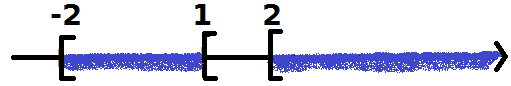
\includegraphics[width=5cm]{1ex1.png}
\end{tabularx}
\end{EX}
}}

\newpage \setcounter{EXO}{0}
\noindent\begin{minipage}{.20\linewidth}\begin{center}                  
\noindent \emph{Lycée Paul Lapie - Courbevoie}
\end{center}\end{minipage}
\begin{minipage}{1.5\linewidth}\begin{center}	
\noindent \cl\\ Chapitre 1
\end{center}\end{minipage}

\begin{center}\shadowbox{ \Large Planche n°1 (bis)  : \dev } 	
\end{center}
{\large{


\begin{EX} 
Résoudre les équations bicarrées suivantes : 
\begin{enumerate}
\renewcommand{\tabularxcolumn}[1]{b{#1}}
\begin{tabularx}{\linewidth}{XX}	
\item $x^4-6x^2+8=0$&
\item $2x^4-6x^2-8=0$ \\
\item $x^4-2x^2-3=0$&
\item $x^4+9x^2+20=0$\\
\end{tabularx}
\end{enumerate}
\end{EX}

\begin{EX} 
Déterminer la fonction polynôme du second degré dont la courbe passe par les points 
$$A(2\,;\,4) \hspace{1.5cm} B(4\,;\,2) \hspace{1.5cm} C(6\,;\,-4)$$
\end{EX}

\begin{EX} 
Déterminer la fonction polynôme du second degré dont la courbe passe par les points 
$$A(1\,;\,1) \hspace{1.5cm} B(-1\,;\,5) \hspace{1.5cm} C(3\,;\,13)$$
\end{EX}

\begin{EX} 
Déterminer la fonction polynôme du second degré dont la courbe passe par les points 
$$A(1\,;\,1) \hspace{1.5cm} B(3\,;\,5) \hspace{1.5cm} C(0\,;\,2)$$
\end{EX}

\begin{EX} 
Donner l'ensemble de définition des fonctions suivantes :
\begin{enumerate}
\renewcommand{\tabularxcolumn}[1]{b{#1}}
\begin{tabularx}{\linewidth}{XX}	
\item $f(x)=\f{x-3}{x^2+x+1}$&
\item $g(x)=\f{x^2-2x+2}{2x^4-6x^2-8}$ \\
\item $h(x)=\f{x-4}{-x^2+5x+6}$&
\item $k(x)=\f{x}{x^2-x+2}$\\
\end{tabularx}
\end{enumerate}
\end{EX}

\begin{EX} 
Faire les tableaux de signes des fonctions précédentes.
\end{EX}

\begin{EX} Déterminer les coordonnées des (éventuels) points d'intersection des courbes $\mathcal{C}_1$ et $\mathcal{C}_2$ : 
$$ \mathcal{C}_1 \, : \, y=\f{x-1}{x+2} \hspace{2cm} \mathcal{C}_2 \, : \, y=-x+3$$
~~

$$ \mathcal{C}_1 \, : \, y=\f{x^2}{2x+2} \hspace{2cm} \mathcal{C}_2 \, : \, y=x-1$$
\end{EX}
}}





\newpage \setcounter{EXO}{0} 
\def\dev{\Large Suites numériques }
\noindent\begin{minipage}{.20\linewidth}\begin{center}                  
\noindent \emph{Lycée Paul Lapie - Courbevoie}
\end{center}\end{minipage}
\begin{minipage}{1.5\linewidth}\begin{center}	
\noindent \cl\\ Chapitre 2
\end{center}\end{minipage}

\begin{center}\shadowbox{ \Large Planche n°2  : \dev } 	
\end{center}

\begin{EX} Soit la suite $(u_n)$ définie pour tout entier naturel $n$ par $u_n=2n^2-1$. \\
Calculer $u_0$, $u_1$, $u_2$ et $u_{10}$.
\end{EX}
\begin{EX} Soit la suite $(v_n)$ définie pour tout entier naturel $n$ non nul par $v_n=\f{n+1}{n}$. \\
Calculer $v_1$, $v_2$, $v_3$ et $v_{10}$.
\end{EX}
\begin{EX} Soit la suite $(w_n)$ définie pour tout entier naturel $n$ par $w_0=1$ et $w_{n+1}=3w_n-4$. \\
Calculer $w_1$, $w_2$, $w_3$. Comment faire pour calculer $w_{10}$ ?
\end{EX}
\begin{EX} On considère la suite de triangles rectangles isocèles suivante : le premier triangle a ses côtés de longueur 1, 1 et $\sqrt2$. On effectue un agrandissement de rapport 3 pour obtenir le triangle suivant. \begin{enumerate}
\item Construire les 3 premier triangles.
\item Calculer les périmètres $p_1$, $p_2$ et $p_3$ des trois premiers triangles. \\
Donner la relation entre $p_{n+1}$ et $p_n$. 
\item Calculer les aires $a_1$, $a_2$ et $a_3$ des trois premiers triangles. \\
Donner la relation entre $a_{n+1}$ et $a_n$. 
\end{enumerate}
\end{EX}
\begin{EX}Pour chacune des suites suivantes, indiquer si elle est définie par une formule explicite ou par une relation de récurrence, puis déterminer/calculer les 3 premiers termes, puis le 5ème. 
\begin{itemize}
\item[•] $~~\forall n \in \mathbb{N}~:~~a_n=3n^2$.
\item[•] $~~\forall n \in \mathbb{N}~:~~b_n=n-1$.
\item[•] $~~\forall n \in \mathbb{N}~:~~\left \{ \begin{array}{l}
c_0=-2		 \\           			
c_{n+1}=c_n-5	 
\end{array} \right.$
\item[•] $~~\forall n \in \mathbb{N}^*~:~~\left \{ \begin{array}{l}
d_1=-2		 \\           			
d_{n+1}=\f{1}{2}d_n	 
\end{array} \right.$
\item[•] $~~\forall n \in \mathbb{N}^*~:~~e_n=4$
\item[•] $~~\forall n \in \mathbb{N}~:~~\left \{ \begin{array}{l}
f_0=1		 \\           			
f_{n+1}=3f_n+2n^2-1	 
\end{array} \right.$
\end{itemize}
\end{EX}
\begin{EX} Les algorithmes ci-dessous permettent de calculer le terme de rang $n$ de trois suites. \\
Indiquer le premier terme et la relation de récurrence ou la formule explicite définissant chacune de ces suites.\\

\begin{Sbox}\begin{minipage}{0.25\linewidth}
$u \leftarrow -4$ \\
Pour $k$ allant de 1 à $n$ faire

~\qquad  $u \leftarrow u+5$
\end{minipage}\end{Sbox} \fbox{\TheSbox} \qquad \begin{Sbox}\begin{minipage}{0.25\linewidth}
$v \leftarrow 300$ \\
Pour $k$ allant de 1 à $n$ faire

~\qquad  $v \leftarrow 2v$
\end{minipage}\end{Sbox} \fbox{\TheSbox} \qquad \begin{Sbox}\begin{minipage}{0.25\linewidth}
Pour $k$ allant de 1 à $n$ faire

~\qquad  $w \leftarrow \sqrt{2k+5}$
\end{minipage}\end{Sbox} \fbox{\TheSbox} \\
~~\\

\begin{Sbox}\begin{minipage}{0.25\linewidth}
$t \leftarrow 0$ \\
Pour $k$ allant de 1 à $n$ faire

~\qquad  $t \leftarrow k+3t$
\end{minipage}\end{Sbox} \fbox{\TheSbox} \qquad \begin{Sbox}\begin{minipage}{0.25\linewidth}
Pour $k$ allant de 0 à $n$ faire

~\qquad  $s \leftarrow \f{3k+1}{k+2}$
\end{minipage}\end{Sbox} \fbox{\TheSbox} \qquad \begin{Sbox}\begin{minipage}{0.25\linewidth}
$r \leftarrow 0$ \\
Pour $k$ allant de 0 à $n$ faire

~\qquad  $r \leftarrow 2k-5r+1$
\end{minipage}\end{Sbox} \fbox{\TheSbox}
\end{EX}

\newpage

\noindent\begin{minipage}{.20\linewidth}\begin{center}                  
\noindent \emph{Lycée Paul Lapie - Courbevoie}
\end{center}\end{minipage}
\begin{minipage}{1.5\linewidth}\begin{center}	
\noindent \cl\\ Chapitre 2
\end{center}\end{minipage}

\begin{center}\shadowbox{ \Large Planche n°2 (bis) : \dev } 	
\end{center}

\begin{EX} Pour les suites suivantes, préciser si c'est une suite définie par une formule explicite ou une relation de récurrence, puis calculer les 4 premiers termes. 
$$ \textbf{a.} ~~\forall n \in \mathbb{N}~:~~\left \{ \begin{array}{l}
u_0=1		 \\           			
u_{n+1}=\sqrt{2u_n}		 
\end{array} \right. \hspace{1.5cm}  
\textbf{b.} ~~\forall n \in \mathbb{N}^*~:~~\left \{ \begin{array}{l}
u_1=-1		 \\           			
u_{n+1}=2u_n+1		 
\end{array} \right. \hspace{1.5cm}  
\textbf{c.} ~~\forall n \in \mathbb{N}~:~~u_n=\f{n}{n+1}  $$  
$$ \textbf{d.} ~~\forall n \in \mathbb{N}~:~~\left \{ \begin{array}{l}
u_0=1		 \\           			
u_{n+1}=3u_n-4n-1		 
\end{array} \right. \hspace{0.5cm}  
\textbf{e.} ~~\forall n \in \mathbb{N}^*~:~~\left \{ \begin{array}{l}
u_0=2		 \\           			
u_{n}=\f{u_{n-1}}{	2u_{n-1}+1}	 
\end{array} \right.  \hspace{0.5cm} 
\textbf{f.} ~~\forall n \in \mathbb{N}^*~:~~\left \{ \begin{array}{l}
u_0=2		 \\           			
u_{n}=2u_{n-1}+n^2 	 
\end{array} \right. $$

\end{EX}

\begin{EX}
On considère la suite $(u_n)$ suivante : 
$$\forall n \in \mathbb{N}~:~~\left \{ \begin{array}{l}
u_0=0	 \\           			
u_{n+1}=\sqrt{2u_n+3}		 
\end{array} \right.$$
\begin{enumerate}
\item Dans un repère du plan, on a représenté la courbe de la fonction $f : x \ass \sqrt{2x+3}$ . \\
Sur l'axe des abscisses, en utilisant les courbes proposées, construire les 4 premiers termes de la suite.
\begin{center}
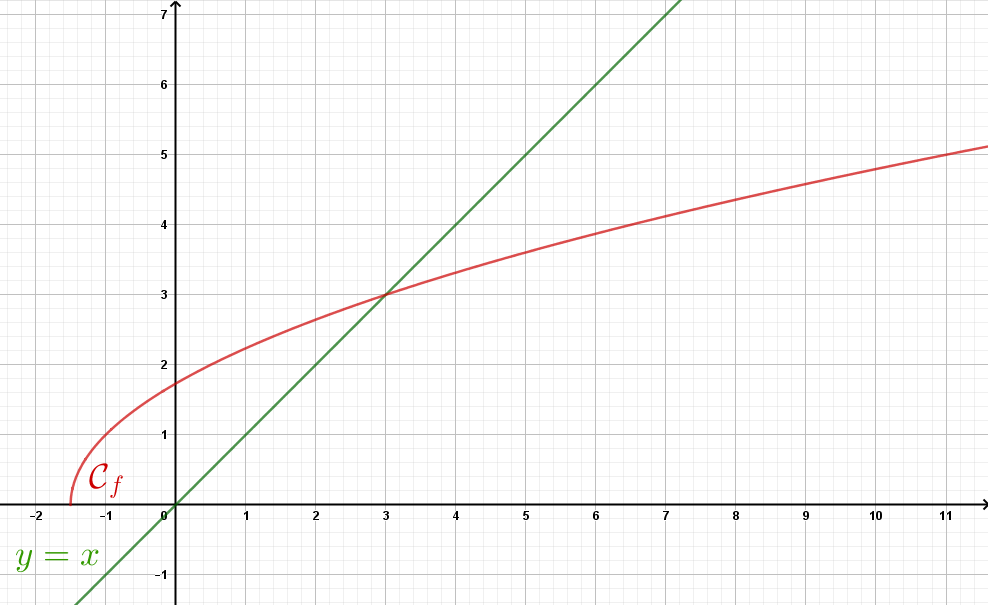
\includegraphics[width=12cm]{2exo1.png}
\end{center}
\item Conjecturer le sens de variations de la suite $(u_n)$. 
\item Conjecturer la limite de $(u_n)$ lorsque $n$ tend vers $+\infty$.

\item Mêmes questions pour $u_0=11$.
\end{enumerate}

\end{EX}

\begin{EX} 
Pour les suites suivantes : 
\begin{enumerate}
\item Conjecturer le sens de variations en calculant les premiers termes.
\item Démontrer les conjectures.
\item Représenter la suite dans un repère.
\item Conjecturer la limite éventuelle des suites.
\end{enumerate}
$$ \textbf{a.} ~~\forall n \in \mathbb{N}~:~~ u_{n}=-n^2+7n+8  \hspace{1.5cm}  
\textbf{b.} ~~\forall n \in \mathbb{N}^*~:~~u_{n}=0.5n^3-3n^2+n-1  \hspace{1.5cm}  
\textbf{c.} ~~\forall n \in \mathbb{N}~:~~u_n=\f{n-1}{n+1}  $$  


\end{EX}


\newpage \setcounter{EXO}{0}

\noindent\begin{minipage}{.20\linewidth}\begin{center}                  
\noindent \emph{Lycée Paul Lapie - Courbevoie}
\end{center}\end{minipage}
\begin{minipage}{1.5\linewidth}\begin{center}	
\noindent \cl\\ Chapitre 2
\end{center}\end{minipage}

\begin{center}\shadowbox{ \Large Planche n°2 (ter) : \dev } 	
\end{center}


\begin{EX} On considère la suite arithmétique $(u_n)$ de raison $r=13$ et de premier terme $u_0=-8$. \begin{enumerate}
\item Calculer $u_1$, $u_2$ et $u_3$. 
\item Donner la relation de terme général de $u_n$.
\item Calculer $u_{12}$.
\end{enumerate}
\end{EX}

\begin{EX} On considère la suite arithmétique $(u_n)$ telle que $u_{4}=15$ et $u_{23}=41$. \\
Déterminer la raison et le premier terme $u_0$. 
\end{EX}


\begin{EX} On considère la suite arithmétique $(u_n)$ telle que $u_{8}=15$ et $u_{12}=25$. \\
Déterminer la raison et le premier terme $u_0$. 
\end{EX}


\begin{EX} On considère la suite géométrique $(v_n)$ de raison $q=\f{3}{2}$ et de premier terme $v_0=1$. \begin{enumerate}
\item Calculer $v_1$, $v_2$ et $v_3$. 
\item Donner la relation de terme général de $v_n$.
\item Calculer $v_{12}$.
\end{enumerate}
\end{EX}

\begin{EX} On considère la suite géométrique $(w_n)$ positive telle que $w_{4}=162$ et $w_{6}=1458$. \\
Déterminer la raison et le premier terme $w_0$. 
\end{EX}

\begin{EX} On considère la suite géométrique $(v_n)$ positive telle que $v_{3}=6$ et $v_{8}=1458$. \\
Déterminer la raison et le premier terme $v_0$. 
\end{EX}

\begin{EX} On considère la suite géométrique $(v_n)$ positive telle que $v_{10}=15$ et $v_{15}=46875$. \\
Déterminer la raison et le premier terme $v_0$. 
\end{EX}

\begin{EX} Calculer les sommes :
$$S=1+2+3+4+...+75 \hspace{3cm} T=2+4+6+8+...+142 \hspace{3cm} R= 7+10+13+16+...58$$
\end{EX}

\begin{EX} 
Calculer les sommes :
$$ S = 1+4+16+...+262144 \hspace{3cm} T=3-6+12-24+...+192 \hspace{2.5cm} R=9+3+1+\f{1}{3}+...+\f{1}{729}$$
\end{EX}



\newpage \setcounter{EXO}{0} 
\def\dev{\Large Suites numériques }

\noindent\begin{minipage}{.20\linewidth}\begin{center}                  
\noindent \emph{Lycée Paul Lapie - Courbevoie}
\end{center}\end{minipage}
\begin{minipage}{1.5\linewidth}\begin{center}	
\noindent \cl\\ Chapitre 2
\end{center}\end{minipage}

\begin{center}\shadowbox{ \Large Planche n°2 (quater) : \dev } 	
\end{center}



\begin{EX}
$(u_n)$ est une suite définie par $u_0=2$ et pour tout entier naturel $n$, $u_{n+1}=2u_n+5$. 
\begin{enumerate}
\item Calculer $u_1 \,;\, u_2 \,;\, u_3\,;\,u_4 \,;\,u_5$. La suite $(u_n)$ est-elle arithmétique ? Géométrique ?
\item Pour tout entier naturel $n$ on pose $w_n=u_n+5$. Calculer $w_1 \,;\,w_2 \,;\, w_3\,;\,w_4 \,;\,w_5$.
\item Démontrer que la suite $(w_n)$ est géométrique.
\item Exprimer $w_n$, puis $u_n$ en fonction de $n$.
\end{enumerate} 
\end{EX}

\begin{EX}
Soit la suite $(u_n)$ définie par $u_0= \f{1}{2}$ et $u_{n+1}=\f{u_n}{1+2u_n}$.
\begin{enumerate}
\item Calculer $u_1 \,;\, u_2 \,;\, u_3\,;\,u_4 \,;\,u_5$. La suite $(u_n)$ est-elle arithmétique ? Géométrique ?
\item On pose $v_n=\f{1}{u_n}+1$. Prouver que la suite $(v_n)$ est arithmétique. 
\item  Exprimer $v_n$, puis $u_n$, en fonction de $n$.
\end{enumerate}  
\end{EX}

\begin{EX}
$(u_n)$ est la suite définie par $u_0=1$ et $u_{n+1}=\f{1}{2} u_n + \f{1}{4}$.
\begin{enumerate}
\item  Placer sur l'axe des abscisses les termes $u_0\,;\,u_1 \,;\, u_2 \,;\, u_3$. 
\begin{center}
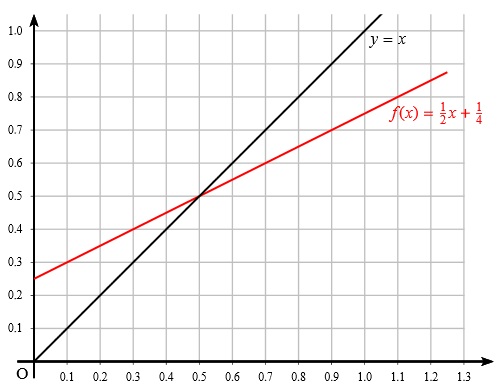
\includegraphics[width=13cm]{2exo_suite_aux.png}
\end{center}
\item Conjecturer alors la limite de la suite $(u_n)$.
\item On pose $v_n=u_n-\f{1}{2}$.
\begin{enumerate}
\item Prouver que la suite $(v_n)$ est géométrique.
\item Exprimer $v_n$, puis $u_n$ en fonction de $n$.
\end{enumerate}
\end{enumerate}
\end{EX}





\newpage \setcounter{EXO}{0} 
\def\dev{\Large Probabilités Conditionnelles }


\noindent\begin{minipage}{.20\linewidth}\begin{center}                  
\noindent \emph{Lycée Paul Lapie - Courbevoie}
\end{center}\end{minipage}
\begin{minipage}{1.5\linewidth}\begin{center}	
\noindent \cl\\ Chapitre 3
\end{center}\end{minipage}

\begin{center}\shadowbox{ \Large Planche n° 3 : \dev } 	
\end{center}

\begin{EX}
Marius achète un hebdomadaire une fois par semaine. Deux fois sur trois il achète l'hebdomadaire $A$; sinon il achète l'hebdomadaire $B$. Toutes les semaines, il fait la grille de mots croisés. Dans l'hebdomadaire $A$, il finit la grille trois fois sur quatre, alors que dans le $B$, plus difficile, il ne la termine qu'une fois sur deux. 

\begin{qu} Traduire toutes les données à l'aide de probabilités, et/ou de probabilités conditionnelles.
\end{qu}
\begin{qu} Représenter la situation par un arbre pondéré.
\end{qu}
\begin{qu} En entrant chez le buraliste, quelle est la probabilité qu' il ressorte avec l'hebdomadaire $B$ et qu'il finisse la grille ?
\end{qu}
\begin{qu} Quelle est la probabilité que Marius réussisse sa grille ?
\end{qu}
\end{EX}
\begin{EX}
\`A un carrefour doté d'un feu tricolore, on a remarqué que :
\begin{itemize}
\item $2\%$ des véhicules s'arrêtent au feu vert,
\item $65\%$ des véhicules s'arrêtent au feu orange (comme le demande le code de la route),
\item $97 \%$ des véhicules s'arrêtent au feu rouge.
\end{itemize}
On décide d'observer le comportement d'un véhicule se présentant au carrefour. On admet que l'état du feu, à l'arrivée du véhicule, est aléatoire, et que la probabilité que le feu soit vert est de $0,6$, celle qu'il soit orange est de $0,1$ et celle qu'il soit rouge est de $0,3$.
\begin{qu} Quelle est la probabilité que le véhicule observé s'arrête ?
\end{qu}
\begin{qu} Le véhicule est passé. Quelle est la probabilité qu'il l'ait fait au feu rouge ?
\end{qu}
\end{EX}
\begin{EX}
On lance deux dés équilibrés. On considère les évènements : \\ A : « la somme est paire »,
B : « en additionnant les deux faces, on a obtenu au moins 6 » et C : « on a obtenu un double. »
\begin{qu} Calculer $P(A)$ , $P(B)$ , $P(C)$ , $P(A\cap B)$ , $P(A\cap C)$ et $P(B\cap C)$
\end{qu}
\begin{qu} En déduire $P_A( B)$ , $P_A(C )$, $P_B(A )$, $P_B(C )$, $P_C(A )$ et $P_C(B )$.
\end{qu}
\end{EX}
\begin{EX}
Lors d’une longue séance de tirs au but, le gardien arrête le 1er tir avec la probabilité 0,3.
\begin{itemize}
\item S’il a arrêté un tir, il arrête le suivant avec la probabilité 0,5 ;
\item S’il a pris un but, il arrête le suivant avec la probabilité 0,2.
\end{itemize}
On admet que tous les tirs sont « cadrés » et l’on note $p_n$ la probabilité que le gardien arrête le n-ième tir ($p_1= 0,3$).

\begin{qu} \`A l’aide d’un arbre de probabilités, montrer que, pour tout $n \se1$, $p_{n+1}=0,3p_n+0,2$.
\end{qu}
\begin{qu} On pose, pour $n\se1$, $u_n=p_n-\displaystyle \frac{2}{7}$. Montrer que la suite $(u_n)$ est géométrique.
\end{qu}
\begin{qu} En déduire $\lim\limits_{n \to +\infty} p_n$. Interpréter le résultat.
\end{qu}
\end{EX}
\begin{EX}
Denis le jardinier entretient le jardin de René. \\
Denis :\og deux fois sur trois, si j'arrose le matin, il pleut le soir!\fg.\\
René : \og oui, mais quand vous n'arrosez pas le matin, c'est-à-dire trois jours sur quatre, il ne pleut pas le soir quatre fois sur cinq! \fg.

Arnaud arrive un soir à l'improviste dans le jardin de René. Quelle est la probabilité qu'il pleuve ?

\end{EX}

\newpage \setcounter{EXO}{0}

\noindent\begin{minipage}{.20\linewidth}\begin{center}                  
\noindent \emph{Lycée Paul Lapie - Courbevoie}
\end{center}\end{minipage}
\begin{minipage}{1.5\linewidth}\begin{center}	
\noindent \cl\\ Chapitre 3
\end{center}\end{minipage}

\begin{center}\shadowbox{ \Large Planche n° 3 (bis) : \dev } 	
\end{center}
\begin{EX}
\begin{qu}
Soit A et B deux évènements indépendants. Montrer qu’il en est de même pour :
\begin{center}\begin{tabular}{p{4cm} p{4cm}p{4cm}}
\textbf{a.~~}$A$ et $\bar{B}$&\textbf{b.~~}$\bar{A}$ et $B$&\textbf{c.~~}$\bar{A}$ et $\bar{B}$\\
\end{tabular}\end{center}
\end{qu}
\begin{qu}
Alfred et Bruno, deux archers tirent simultanément. Les deux évènements A : « Alfred atteint la cible » et B: « Bruno atteint la cible » sont des évènements indépendants de probabilités respectives $\displaystyle \frac{4}{5}$ et $\displaystyle \frac{7}{8}$. \\
Calculer la probabilité des évènements :
\begin{description}
\item [a.] Alfred et Bruno atteignent tous deux la cible.
\item [b.] Seul Alfred atteint la cible.
\item [c.] Aucun des deux n'atteint la cible.
\item [d.] La cible est atteinte.
\item [e.] Un seul archer atteint la cible.
\end{description}
\end{qu}

\end{EX}
\begin{EX}

Le tableau ci-dessous donne la répartition de $150$ stagiaires en fonction de la langue choisie et de l'activité sportive choisie. On choisit un stagiaire au hasard. 

\begin{center}
\begin{tabular}{|p{3cm}| p{3cm}| p{3cm}| p{3cm}|}		
\hline							
 & Tennis & \'Equitation & Voile\\
\hline
Anglais &45 & 18  &27\\
\hline
Allemand &33 & 9 &18 \\
\hline
\end{tabular}
\end{center}
\begin{enumerate}
\item  Les événements \og étudier l'allemand \fg{} et \og pratiquer le tennis \fg{} sont-ils indépendants ?
\item  Les événements \og étudier l'anglais \fg{} et \og pratiquer la voile \fg{} sont-ils indépendants ?
\end{enumerate}

\end{EX}
\begin{EX}

Votre voisine a deux enfants dont vous ignorez le sexe. On considère les événements suivants :
\begin{itemize}
\item $A$="les deux enfants sont de sexes différents"
\item $B$="l'ainé est une fille"
\item $C$="le cadet est un garçon".
\end{itemize}
Montrer que $A$, $B$ et $C$ sont deux à deux indépendants, mais ne sont pas mutuellement indépendants. $ \big( $ie : $p(A \cap B \cap C) \ne p(A) \x p(B) \x p(C) \big).$


\end{EX}
\begin{EX}

\begin{enumerate}
\item Une urne contient 12 boules numérotées de 1 à 12. On en tire une hasard, et on considère les événements 
\begin{center}
$A=\textrm{"tirage d'un nombre pair''}, \qquad B=\textrm{"tirage d'un multiple de 3''}.$
\end{center}
Les événements $A$ et $B$ sont-ils indépendants?
\item Reprendre la question avec une urne contenant 13 boules.
\end{enumerate}

\end{EX}

\newpage \setcounter{EXO}{0}

\noindent\begin{minipage}{.20\linewidth}\begin{center}                  
\noindent \emph{Lycée Paul Lapie - Courbevoie}
\end{center}\end{minipage}
\begin{minipage}{1.5\linewidth}\begin{center}	
\noindent \cl\\ 
\end{center}\end{minipage}

\begin{center}\shadowbox{ \Large Type Bac : \dev } 	
\end{center}
\normalsize

\begin{EX}
\emph{Les probabilités seront arrondies au dix millième.}

\medskip
L'élève part tous les jours à 7~h~40 de son domicile et doit arriver à 8~h~00 à son lycée. Il prend le vélo 7 jours sur 10 et le bus le reste du temps.

Les jours où il prend le vélo, il arrive à l'heure dans $99,4\%$ des cas et lorsqu'il prend le bus, il arrive en retard dans $5\,\%$ des cas.

On choisit une date au hasard en période scolaire et on note $V$ l'évènement 
\og L'élève se rend au lycée à vélo \fg, $B$ l'évènement \og l'élève se rend au lycée en bus \fg{} et $R$ l'évènement \og L'élève arrive en retard au lycée\fg.
\begin{enumerate}
\item Traduire la situation par un arbre de probabilités.
\item Déterminer la probabilité de l'évènement $V \cap R$.
\item Démontrer que la probabilité de l'évènement $R$ est $0,0192$.
\item Un jour donné, l'élève est arrivé en retard au lycée. Quelle est la probabilité qu'il s'y soit rendu en bus?
\end{enumerate}
\hfill \emph{D'après Liban juin 2014.}
\end{EX}


\begin{EX}
\emph{Les résultats seront arrondis à $10^{-4}$ près}

\medskip
 
Un ostréiculteur élève deux espèces d'huîtres : \og la plate \fg{} et \og la japonaise \fg. Chaque année, les huîtres plates représentent 15\,\% de sa production.
 
Les huîtres sont dites de calibre \no 3 lorsque leur masse est comprise entre 66~g et 85~g.
 
Seulement 10\,\% des huîtres plates sont de calibre \no 3, alors que 80\,\% des huîtres japonaises le sont.

\medskip
 
Le service sanitaire prélève une huître au hasard dans la production de l'ostréiculteur. On suppose que toutes les huitres ont la même chance d'être choisies.
 
On considère les évènements suivants : 

\setlength\parindent{8mm}
\begin{itemize}
\item[$\bullet~~$] $J$ : \og l'huître prélevée est une huître japonaise \fg, 
\item[$\bullet~~$] $C$ : \og l'huître prélevée est de calibre \no 3 \fg.
\end{itemize}
\setlength\parindent{0mm}
 
	\begin{enumerate}
		\item Construire un arbre pondéré complet traduisant la situation. 
		\item Calculer la probabilité que l'huître prélevée soit une huître plate de calibre \no 3. 
		\item Justifier que la probabilité d'obtenir une huître de calibre \no 3 est $0,695$. 
		\item Le service sanitaire a prélevé une huître de calibre \no 3. 
Quelle est la probabilité que ce soit une huître plate ?
	\end{enumerate} 

\hfill \emph{D'après Antilles-Guyane juin 2014.}
\end{EX}


\begin{EX}
\medskip 

Une entreprise produit 40\,\% de ballons de football de petite taille et 60\,\% de ballons de taille standard. 

On admet que 2\,\% des ballons de petite taille et 5\,\% des ballons de taille standard ne sont pas conformes à la réglementation. On choisit un ballon au hasard dans l'entreprise. 

On considère les évènements : 

$A$ : \og le ballon de football est de petite taille \fg, 

$B$ : \og le ballon de football est de taille standard \fg, 

$C$ : \og le ballon de football est conforme à la réglementation\fg{} et $\overline{C}$, l'évènement contraire de $C$. 

\medskip

\begin{enumerate}
\item Représenter cette expérience aléatoire à l’aide d’un arbre de probabilité.
\item Calculer la probabilité que le ballon de football soit de petite taille et soit conforme à la règlementation.
\item Montrer que la probabilité de l'événement $C$ est égale à $0,962$.
\item Le ballon de football choisi n'est pas conforme à la réglementation. Quelle est la probabilité que ce ballon soit de petite taille ? On arrondira le résultat à $10^{- 3}$.
\end{enumerate}

\hfill \emph{D'après Amérique du Sud novembre 2014.} 
\end{EX}




\newpage \setcounter{EXO}{0} 
\def\dev{\Large Nombre dérivé et tangente à une courbe }

\noindent\begin{minipage}{.20\linewidth}\begin{center}                  
\noindent \emph{Lycée Paul Lapie - Courbevoie}
\end{center}\end{minipage}
\begin{minipage}{1.5\linewidth}\begin{center}	
\noindent \cl\\ Chapitre 4
\end{center}\end{minipage}

\begin{center}\shadowbox{ \Large Planche n°4  : \dev } 	
\end{center}

\begin{EX}

\renewcommand{\tabularxcolumn}[1]{b{#1}}
\begin{tabularx}{\linewidth}{Xc}	
On considère la fonction définie sur $\mathbb{R}$ par : 
$$f(x)=x^2+3x-1$$Ci-contre la courbe représentative de $f$ dans un repère du plan. \vspace{0.5cm}
\begin{enumerate}
\item Justifier que $f$ est dérivable en $x=2$, puis donner la valeur de $f'(2)$. \vspace{0.5cm}
\item Déterminer l'équation de la tangente $T_{2}$ à $f$ au point d'abscisse $a=2$. \vspace{0.5cm}
\item Dans le repère ci-dessous, tracer la tangente $(T_2)$.
\end{enumerate}

&
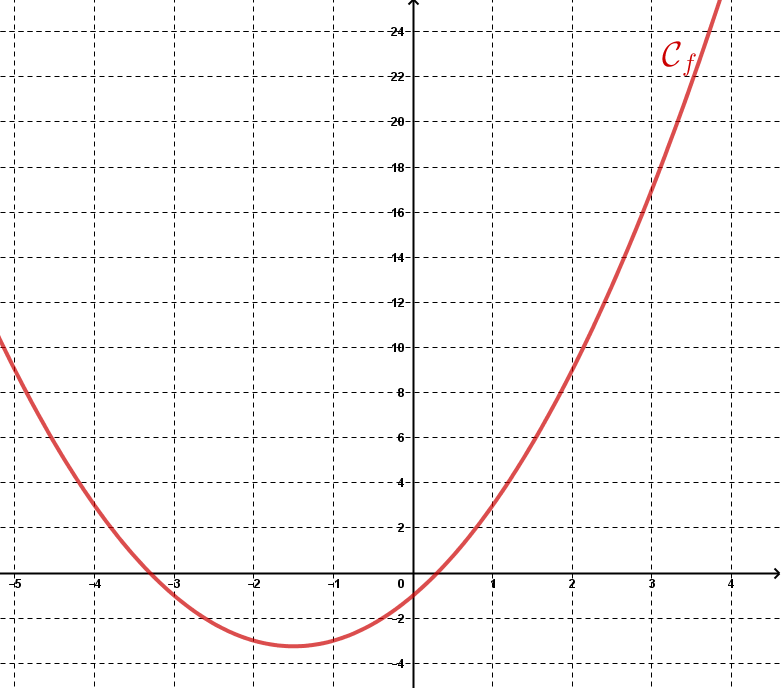
\includegraphics[width=11cm]{4ex1.png}
\end{tabularx}

\end{EX}
\begin{EX}
Dans le repère ci-dessous, on a tracé la courbe de la fonction $f$, ainsi que des tangentes à la courbe $\mathcal{C}_f$ aux points d'abscisses $a=-1$ $a=0$ et $a=2$.
\begin{center}

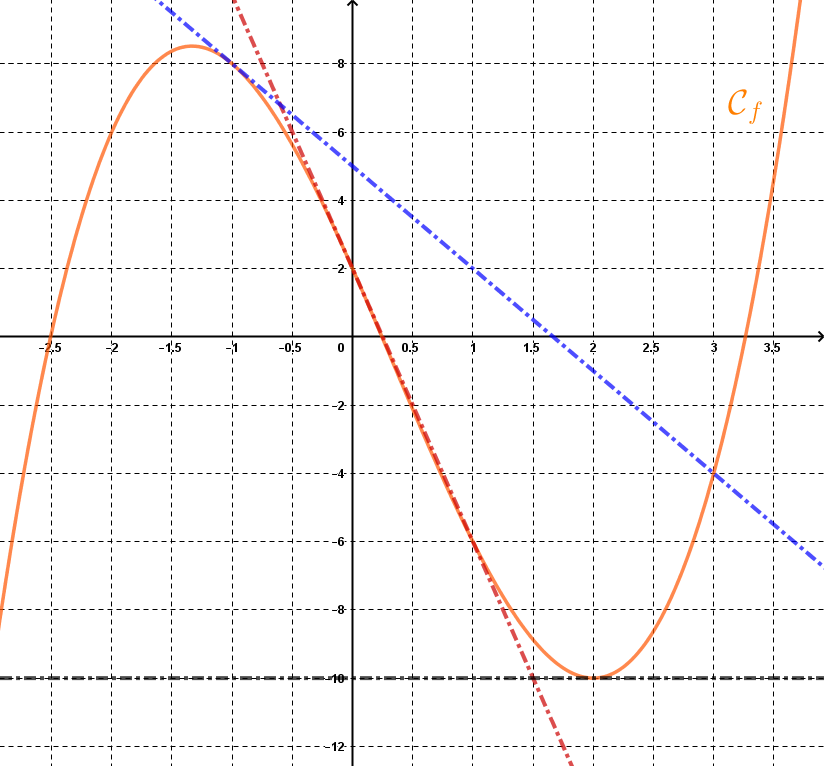
\includegraphics[width=10cm]{4ex2.png}
\end{center}
\begin{enumerate}
\item Lire graphiquement les données suivantes : 
$$f(-1) \qquad f'(-1) \qquad f(0) \qquad f'(0) \qquad f(2) \qquad f'(2)$$
\item Donner les équations des 3 tangentes représentées ci-dessus.
\end{enumerate}

\end{EX}

Exercices du livre : ex 19 + 20 + 23 + 24 + 36 + 41 + 42 + 44 + 45 p 119 ; 120 ; 121.

\newpage

\noindent\begin{minipage}{.20\linewidth}\begin{center}                  
\noindent \emph{Lycée Paul Lapie - Courbevoie}
\end{center}\end{minipage}
\begin{minipage}{1.5\linewidth}\begin{center}	
\noindent \cl\\ Chapitre 4
\end{center}\end{minipage}

\begin{center}\shadowbox{ \Large Planche n°4 (bis) : \dev } 	
\end{center}

\begin{EX}
On dit qu'un corps est en chute libre lorsqu'il est lâché sans vitesse initiale depuis un point et qu'il n'est soumis qu'à son poids (on néglige les frottements de l'air). 

Le corps parcourt alors en $t$ secondes une distance que l'on peut approcher par $d(t)=5t^2$ (mètre).
\begin{enumerate}
\item Quelle est la distance parcourue par le corps en chute libre en 10 secondes ?
\item Pour $h \ne 0$, calculer la vitesse moyenne du corps entre les instants $t=10$ et $t=10+h$. 
\item On définit la \textbf{vitesse instantanée} comme la limite de la vitesse moyenne lorsque $h$ se rapproche de $0$.\\ Déterminer la vitesse instantanée du corps à l'instant $t=10$. 
\item Reprendre les questions pour l'instant $t=5$. 
\end{enumerate} 
\end{EX}

\begin{EX}
Une entreprise fabrique des clous. Le coût de fabrication de $x$ clous ($x$ est exprimé en centaines) est modélisé par la fonction $C$ définie sur $[0\,;\,+\infty[$ par :
$$C(x)=0,3x^2+x+1$$
où $C(x)$ est exprimé en centaine d'euros.
\begin{enumerate}
\item Calculer le coût de fabrication de $1~000$ clous. 
\item On appelle \textbf{coût marginal} pour $q$ unités produites le coût de fabrication d'une unité supplémentaire.\\ Calculer le coût marginal pour $1~000$ clous fabriqués. \\ {\emph{Cela correspond au coût de 1001 unités moins le coût de 1000unités ).}}
\item Démontrer que $C$ est dérivable en $10$ et calculer $C'(10)$.
\item Comparer au résultat précédent.
\end{enumerate}
\end{EX}

\begin{EX} On considère la fonction $f$ définie sur $\mathbb{R}$ par $$f(x)=x^2-2x-1$$
On admet que $f'(0)=-2$ , $f'(1)=0$ et $f'(3)=4$.
\begin{enumerate}
\item Dans un repère orthonormé, tracer la courbe représentative de $f$ et construire les tangentes à la courbe aux points d'abscisses $0$, $1$, et $3$.
\item Déterminer graphiquement les équations des tangentes aux points d'abscisses $0$ et $1$. 
\item Déterminer par le calcul l'équation de la tangente au point d'abscisses $3$.
\end{enumerate}
\end{EX}

\begin{EX}

\renewcommand{\tabularxcolumn}[1]{b{#1}}
\begin{tabularx}{\linewidth}{Xc}	
On considère la fonction $f$ définie sur $\mathbb{R}$ par : $$f(x)=x^3-2x+1$$
On a représenté la courbe de $f$ dans un repère du plan, ainsi que deux tangentes $T_{-1}$ et $T_1$ aux points d'abscisses respectives $-1$ et $1$.

\vspace{1.5cm}

Quelle conjecture peut-on faire sur les droites $T_{-1}$ et $T_1$ ?

 \vspace{0.5cm}
Démontrer cette conjecture.
&
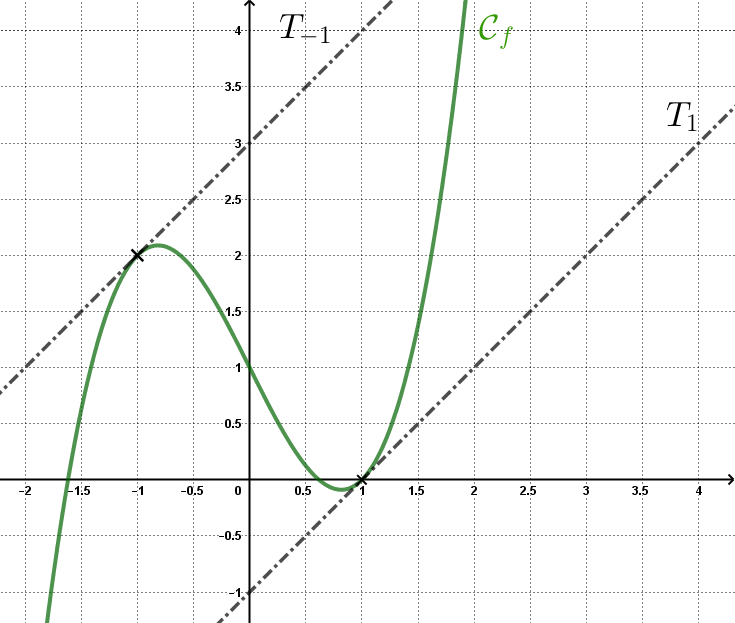
\includegraphics[width=10cm]{4ex5.png}

\end{tabularx} 

\end{EX}




\newpage \setcounter{EXO}{0} 
\def\dev{\Large Trigonométrie }
\def\numero{5}


\noindent\begin{minipage}{.20\linewidth}\begin{center}                  
\noindent \emph{Lycée Paul Lapie - Courbevoie}
\end{center}\end{minipage}
\begin{minipage}{1.5\linewidth}\begin{center}	
\noindent \cl\\ Chapitre \numero
\end{center}\end{minipage}

\begin{center}\shadowbox{ \Large Planche n°\numero  : \dev } 	
\end{center}

\begin{EX}
Parmi les valeurs suivantes, quelles sont celles qui repèrent le même point sur le cercle trigonométrique ?

$$ \f{13\pi}{6} \qquad \f{-13\pi}{6} \qquad \f{11\pi}{6} \qquad -\f{11\pi}{6}  \qquad \f{25\pi}{6} \qquad -\f{\pi}{6}$$ ~~
$$ \f{2\pi}{3} \qquad \f{-\pi}{3} \qquad \f{5\pi}{3} \qquad -\f{5\pi}{3}  \qquad \f{20\pi}{3} \qquad -\f{25\pi}{3}$$

\end{EX}

\begin{EX} On considère le cercle trigonométrique ci-dessous. M est un point image sur le cercle d'un nombre réel $x$. Compléter le tableau suivant avec le signe de $cos(x)$ et $sin(x)$ en fonction de la position de M sur le cercle.


\begin{center}
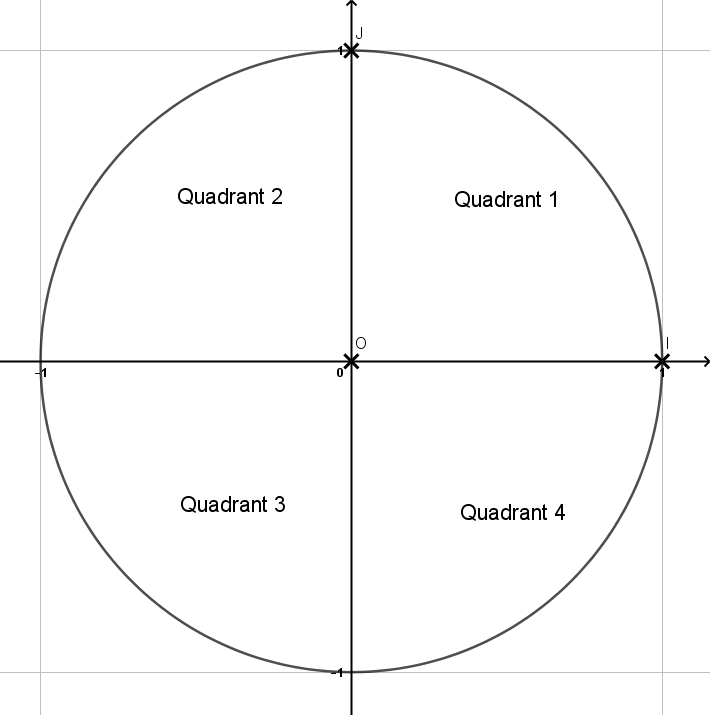
\includegraphics[width=7cm]{5quadrants.png}
~~ \\
\begin{tabular}{|p{4cm}| p{1cm}| p{1cm}| p{1cm}| p{1cm}|}		
\hline							
M est dans le quadrant &1 & 2 & 3& 4\\
\hline
signe de $cos(x)$ & & & &\\
\hline
signe de $sin(x)$ & & & &\\
\hline
\end{tabular}
\end{center}


\end{EX}

\begin{EX}
Pour chacun des réels suivants, dire dans quel quadrant il se trouvera lors de l'enroulement de la droite numérique. Préciser ensuite, si c'est une valeur remarquable, la valeur de son cosinus et de son sinus. 

$$\f{2\pi}{3} \qquad \f{5\pi}{4} \qquad \f{-5\pi}{6} \qquad \f{3\pi}{8} \qquad \f{7\pi}{2} \qquad 9,5 \qquad -\f{13\pi}{4} \qquad \f{11\pi}{6} \qquad -6 \qquad \f{16\pi}{3} \qquad \f{-8\pi}{6} \qquad \f{21\pi}{4}$$

\end{EX}



\begin{EX} Dans chacun des cas suivants, résoudre l'équation proposée dans l'ensemble associé.
\begin{enumerate}
\item $cos(x)=\f{1}{2}$ \\
\textbf{(a.)} \, avec $x \in [0\,;\, \pi]$
\hspace{1.5cm}\textbf{ (b.)} \, avec $x \in [-\f{\pi}{2}\,;\,0]$
\hspace{1.5cm} \textbf{(c.) }\, avec $x \in [-\pi\,;\, \pi]$

\item $sin(x)=\f{-\sqrt3}{2}$ \\
\textbf{(a.)} \, avec $x \in [0\,;\, \pi]$
\hspace{1.5cm}\textbf{ (b.)} \, avec $x \in [-\pi\,;\,-\f{\pi}{2}]$
\hspace{1.5cm} \textbf{(c.) }\, avec $x \in [0\,;\, 2\pi]$

\item $cos(x)=0$ \\
\textbf{(a.)} \, avec $x \in [0\,;\, \pi]$
\hspace{1.5cm}\textbf{ (b.)} \, avec $x \in [-\pi\,;\,0]$
\hspace{1.5cm} \textbf{(c.) }\, avec $x \in [0\,;\, 2\pi]$
\end{enumerate}

\end{EX}

\textbf{Exercices du livre }: chapitre n°7 : ex 20, \textbf{24}, \textbf{33}, 43, 53, 60, 61, \textbf{66}, 67 p193-197.


\newpage
\noindent\begin{minipage}{.20\linewidth}\begin{center}                  
\noindent \emph{Lycée Paul Lapie - Courbevoie}
\end{center}\end{minipage}
\begin{minipage}{1.5\linewidth}\begin{center}	
\noindent \cl\\ Chapitre \numero
\end{center}\end{minipage}

\begin{center}\shadowbox{ \Large Planche n°\numero (bis)  : \dev } 	
\end{center}

\begin{EX} On note $f$ la fonction cosinus, et $g$ la fonction sinus. \begin{enumerate}
\item Déterminer les images par $f$ et par $g$ de $\f{3\pi}{4}$.
\item Trouver un antécédent de $\f{\sqrt3}{2}$ par $f$.
\item Trouver tous les antécédents de $0$ par $g$.
\end{enumerate}
\end{EX}



\begin{EX} 
Comparer, sans calculatrice, les nombres suivants : $$cos(1) \qquad et \qquad cos(2)$$
$$sin(-1) \qquad et \qquad sin(2)$$
$$ cos(\f{17\pi}{8}) \qquad et \qquad cos(\f{\pi}{4})$$
\end{EX}



\begin{EX} 
Résoudre les inéquations suivantes dans l'intervalle $[0\,;\,2\pi]$ :
$$cos(x)\se 0 \hspace{2cm} sin(x)\ie \f{1}{2}  \hspace{2cm} -\f{\sqrt2}{2}\ie cos(x)\ie \f{\sqrt2}{2} \hspace{2cm} -\f{\sqrt2}{2} < sin(x) < \f{\sqrt2}{2} $$
\end{EX}



\begin{EX} 
Résoudre dans \R les équations suivantes : 
$$(1) \qquad cos(x)=\f{-\sqrt3}{2}$$
~~
$$(2) \qquad 2sin(x)-1=0$$
~~
$$(3) \qquad \big( 2cos(x)-1 \big) \big( sin(x)+1 \big) =0$$
~~
$$(4) \qquad \big( cos(x)-1 \big) \big( \sqrt2\,sin(x)+1 \big) =0$$
\end{EX}



\begin{EX} Résoudre dans $[-\pi\,;\, \pi]$ les inéquations suivantes : (on pourra s'aider d'un tableau de signes)
$$sin(x)cos(x) \ie 0$$
~~
$$ cos(x) \big( \sqrt2 sin(x)-1 \big) \se 0$$
~~
$$ \big(2sin(x)-\sqrt3 \big) \big(1-2cos(x) \big) > 0 $$
\end{EX}
\vspace{2cm}

\textbf{Exercices du livre }: chapitre n°8 : ex 40, 42, 43, 44, 49, 52, 66, 67, 69 p215-225.





\newpage \setcounter{EXO}{0} 
\def\dev{\Large Fonction dérivée }
\def\numero{6}

\noindent\begin{minipage}{.20\linewidth}\begin{center}                  
\noindent \emph{Lycée Paul Lapie - Courbevoie}
\end{center}\end{minipage}
\begin{minipage}{1.5\linewidth}\begin{center}	
\noindent \cl\\ Chapitre \numero
\end{center}\end{minipage}

\begin{center}\shadowbox{ \Large Planche n°\numero : \dev } 	
\end{center}

\begin{EX}
On considère la fonction $f$ définie sur $I=[-3\,;\,2]$ par : 
$$f(x)=2x^3+3x^2-12x+4$$
\begin{enumerate}
\item Calculer $f'(x)$ et étudier son signe. 
\item Dresser le tableau de variations de $f$ sur $[-3\,;\,2]$.
\item Quel est le maximum de $f$ sur I ? Pour quelle(s) valeur(s) est-il atteint ?
\item  Quel est le minimum de $f$ sur I ? Pour quelle(s) valeur(s) est-il atteint ?
\end{enumerate}

\end{EX}

\begin{EX} Un industriel souhaite fabriquer une boite sans couvercle à partir d'une plaque de métal de 18cm de large et 24cm de long. Pour cela, il enlève des carrés dont la longueur du côté mesure $x$ aux quatre coins de la plaque, et il relève ensuite verticalement pour former les côtés de la boîte. 
\begin{enumerate}
\item On note $V$ la fonction volume de la boite. Quel est l'ensemble de définition de $V$ . Calculer $V(x)$.
\item Pour quelle valeur de $x$ la contenance de la boîte est-elle maximale ?
\item Peut-il construire une boîte dont la contenance est supérieure à $650 cm^3$ ?
\end{enumerate}

\end{EX}

\begin{EX}
On a modélisé l'évolution d'une épidémie de grippe de la façon suivante : si $t$ est le temps (en jour) écoulé depuis le début de l'épidémie, le nombre de cas en millier est donné par : 
$$f(t)=\f{-1}{6}t^3+\f{5}{2}t^2+28t$$
\begin{enumerate}
\item Combien de malades compte-t-on au bout de 5 jours ? de 20jours ?
\item Donner l'expression de la dérivée $f'(t)$. \\
On appelle vitesse instantanée d'évolution au cours du temps $t$ le nombre dérivé de la fonction $f$ en $t$.
\item Déterminer la vitesse instantanée d'évolution de la maladie au début de l'épidémie.
\item Déterminer la vitesse instantanée d'évolution de la maladie à l'instant $t=3$ jours.
\item Déterminer le nombre de jours pour atteindre le pic de l'épidémie.
\item Quelle est la vitesse d'évolution de la maladie au moment du pic ?
\end{enumerate}

\end{EX}

\begin{EX}
ABCD est un carré de côté 1. M est un point du segment $[AB]$. On place le point N tel que CN=AM sur la demi-droite $[BC)$. La droite (MN) coupe (CD) en P. \\
On pose $AM=x$. \\
Le but de l'exercice est de déterminer la position du point M sur $[AB]$ tel que la distance PC soit maximale.
\begin{enumerate}
\item Donner les valeurs de $x$ pour lesquelles la modélisation est possible.
\item Exprimer BM et BN en fonction de $x$.
\item Montrer que : $PC=\f{-x^2+x}{x+1}$.
\item Répondre au problème posé.
\end{enumerate}

\end{EX}






\newpage \setcounter{EXO}{0} 
\def\dev{\Large Produit scalaire }


\noindent\begin{minipage}{.20\linewidth}\begin{center}                  
\noindent \emph{Lycée Paul Lapie - Courbevoie}
\end{center}\end{minipage}
\begin{minipage}{1.5\linewidth}\begin{center}	
\noindent \cl\\ Chapitre 8
\end{center}\end{minipage}

\begin{center}\shadowbox{ \Large Planche n° 8 : \dev } 	
\end{center}

\begin{EX}
ABC est un triangle équilatéral de côté 2, et I est le milieu de $[AB]$. Calculer les produits scalaires suivants :
$$\v{BC}.\v{BA} \hspace{2cm} \v{AI}.\v{AC} \hspace{2cm} \v{BC}.\v{CA} $$

\end{EX}
\begin{EX}
Choisir, dans chacun des cas suivants, l'expression la plus adaptée pour le calcul du produit scalaire $\v{u}.\v{v}$, puis calculez-le. \\
\emph{Une unité de longueur correspond à un carreau.}

\begin{center}
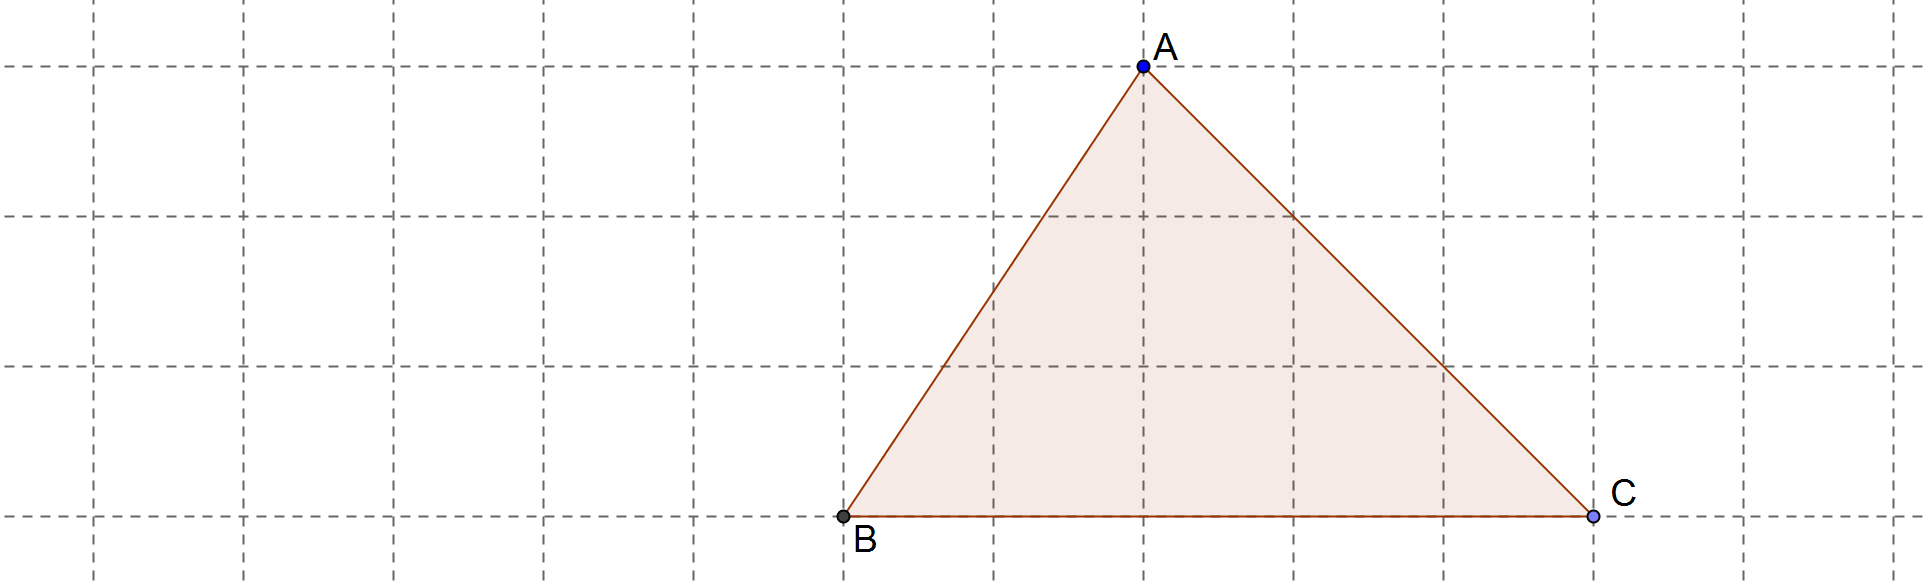
\includegraphics[width=17cm]{8ex1.png}
\end{center}
\end{EX}

\begin{EX} ABCD est un carré de centre O et de côté $a$. Calculer en fonction de $a$ les produits scalaires suivants : 

\begin{enumerate}
\item $\v{CD}.\v{CA}$ \hspace{2cm} $\v{AD}.\v{CB}$ \hspace{2cm} $\v{BD}.\v{AC}$
\item $\v{OB}.\v{AB}$ \hspace{2cm} $\v{OA}.\v{OC}$ \hspace{2cm} $\v{DA}.\v{BD}$
\end{enumerate}

\end{EX}

\begin{EX}
ABCD est un carré de côté $a$. I est le milieu de $[AD]$ et J est le milieu de $[CD]$. 
\begin{enumerate}
\item En décomposant avec la relation de Chasles, calculer $\v{AJ}.\v{BI}$
\item Que peut-on en conclure ?
\end{enumerate}

\end{EX}

\begin{EX}
Dans le plan muni d'un repère orthonormé, on considère trois points A, B et C tels que $\v{AB}\left (\begin{array}{c}
	1 \\
	 -1\\
\end{array} \right) $ et $\v{AC}\left (\begin{array}{c}
	x \\
	 2\\
\end{array} \right)$. \\

En utilisant deux expressions du produit scalaire, déterminer la ou les valeurs de $x$ dans chacun des cas suivants :
\begin{enumerate}
\item $BAC=\f{\pi}{2}$
\item $BAC=\pi$
\item $BAC=\f{\pi}{4}$
\end{enumerate}

\end{EX}

\begin{EX} Dans un repère orthonormé du plan on considère les points
$$M(2\,;\,-2) \hspace{3cm} N(-3\,;\,1) \hspace{3cm} P(1\,;\,2)$$
\begin{enumerate}
\item Calculer $\v{MN}.\v{MP}$.
\item En déduire la valeur exacte de l'angle PMN.
\end{enumerate}

\end{EX}

\begin{EX} 
ABC est un triangle tel que AB=4, AC=6 et BC=7. \\
Calculer à 0,1° près les trois angles de ce triangle.
\end{EX}

\textbf{Exercices du livre }: chapitre 9 : n° 23 à 26, 30, 43, 55, 56 p 243 à 247.






\newpage \setcounter{EXO}{0} 
\def\dev{\Large Variables aléatoires réelles }


\noindent\begin{minipage}{.20\linewidth}\begin{center}                  
\noindent \emph{Lycée Paul Lapie - Courbevoie}
\end{center}\end{minipage}
\begin{minipage}{1.5\linewidth}\begin{center}	
\noindent \cl\\ Chapitre 9
\end{center}\end{minipage}

\begin{center}\shadowbox{ \Large Planche n° 9 : \dev } 	
\end{center}



\begin{EX}
La roue de la fortune ! \\
Le jeu est simple, dans une partie, on fait tourner la roue de loterie ci-contre deux fois de suite, et on gagne à chaque étape le nombre de 
\includegraphics[width=0.8cm]{9mms.png} indiqué par la flèche rouge. \\
\begin{center}
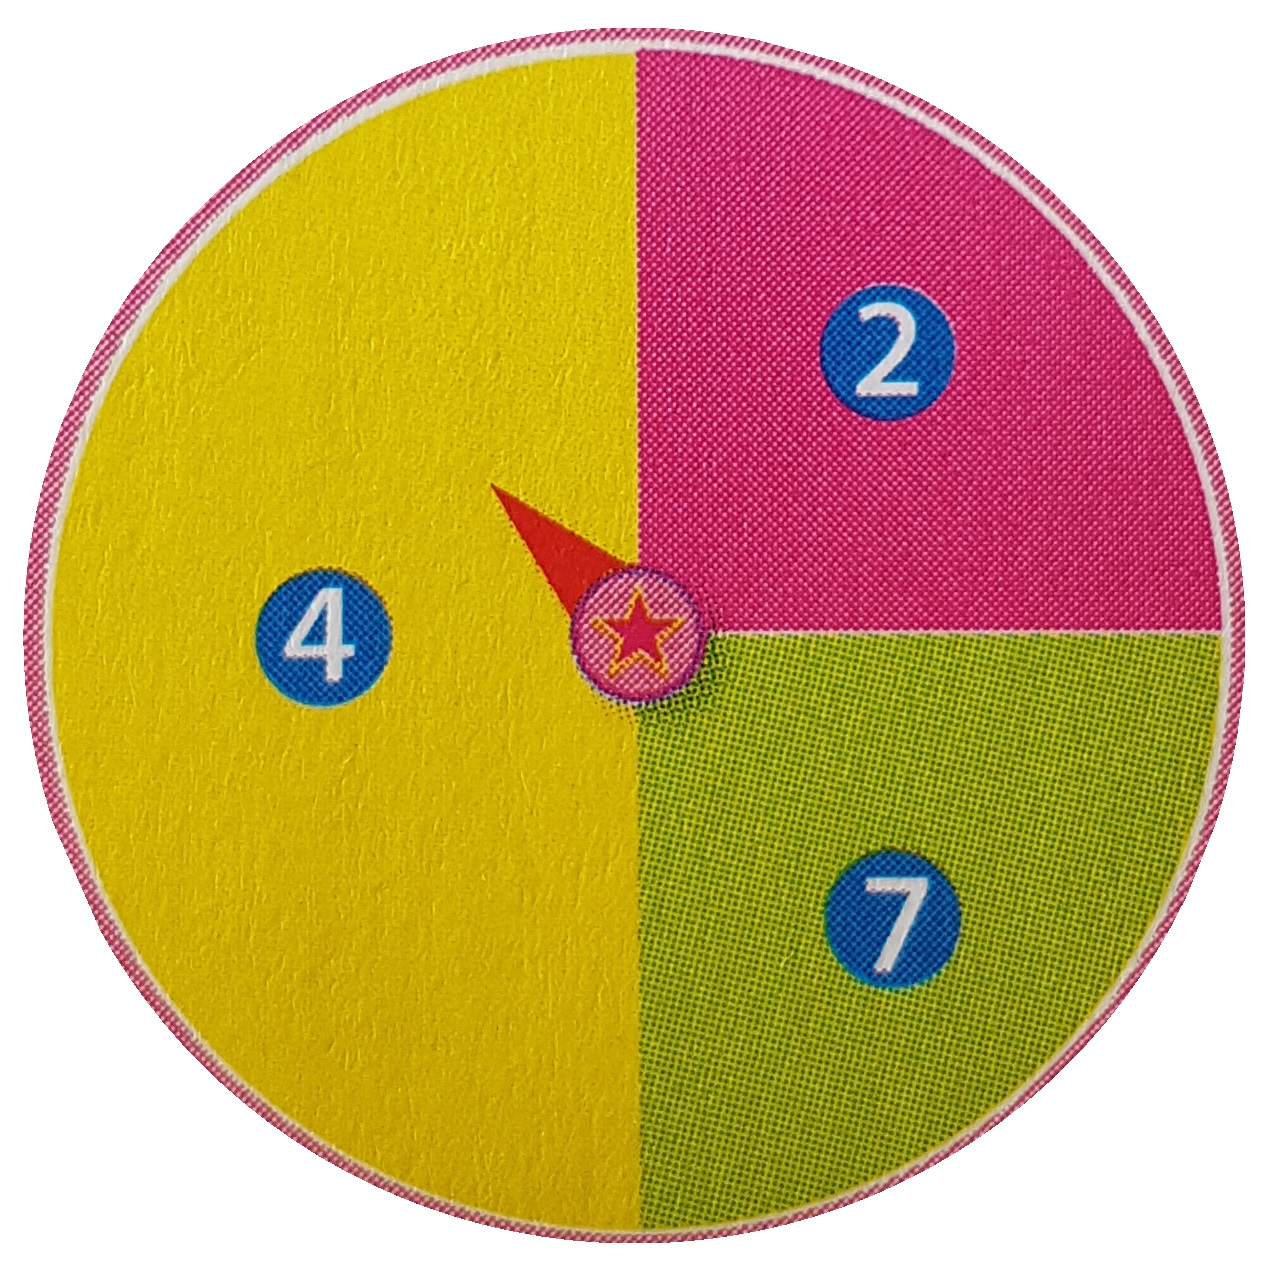
\includegraphics[width=3cm]{9roue.jpg}
\end{center}

Combien peut-on espérer gagner en moyenne de 
\includegraphics[width=0.8cm]{9mms.png} par partie, si on joue un très grand nombre de partie ?

~\hrulefill~

{\small{ {\underline{Indications :}} faire un arbre de probabilité modélisant le nombre de bonbons gagnés après les deux lancers de roue. Définir la variable aléatoire X représentant le nombre de bonbons gagnés après les deux parties. Déterminer la loi de $X$ puis conclure.}}
\end{EX}
\begin{EX}
\`A la boulangerie, Julie demande à la boulangère de choisir au hasard deux beignets. Il y a six beignets à la pomme, cinq beignets choco-noisette et neuf beignets fruits rouges. 

On note $B$ la variable aléatoire égale au nombre de beignets à la pomme choisis. 
\begin{enumerate}
\item Quel est l'ensemble des valeurs prises par la variable aléatoire $B$ ?
\item Calculer $P(B=2)$.
\item Calculer $P(B=1)$.
\item Calculer $P(B \ie 1)$.
\end{enumerate}

\end{EX}

\begin{EX}
Le nombre de caisses en service à midi dans un supermarché donné est une variable aléatoire prenant les valeurs $1\,\;\,2\,\;\,3\,\;\,4$. \\ 
Elle vaut : \begin{itemize}
\item[•] 1 avec la probabilité $0,2$;
\item[•] 2 avec la probabilité $0,3$;
\item[•] 3 avec la probabilité $0,25$;
\end{itemize}
\begin{enumerate}
\item Calculer la probabilité que 4 caisses soient en service à midi dans ce supermarché. 
\item Calculer la probabilité qu'il y ait au moins 2 caisses en service à midi dans ce supermarché.  
\end{enumerate}
\end{EX}

\begin{EX} On lance trois fois de suite une pièce de monnaie équilibrée, et on note les résultats obtenus. Par exemple, (Face ; Face ; Pile) se note FFP. \begin{enumerate}
\item Représenter cette expérience par un arbre de probabilité pondéré.
\item Déterminer la probabilité pour que le troisième lancer de la pièce donne \og Face \fg{} 
\item \`A chaque tirage, on associe 20 points pour \og Pile \fg{} , et 10 points pour \og Face \fg{} . On note $Y$ la somme des points obtenus. \\
Donner la loi de probabilité de $Y$, et calculer son espérance. Interpréter cette valeur.
\end{enumerate}
\end{EX}
Exercices du livre : QCM p 315 ; 46 p 323 ; 48 p 323 ; 53 p 325 ; 58 p 325 ; 71 p 327 ; 78 p 328 ; 82 p 329




\newpage \setcounter{EXO}{0} 

\noindent\begin{minipage}{.20\linewidth}\begin{center}                  
\noindent \emph{Lycée Paul Lapie - Courbevoie}
\end{center}\end{minipage}
\begin{minipage}{1.5\linewidth}\begin{center}	
\noindent \cl\\ Chapitre 10
\end{center}\end{minipage}

\begin{center}\shadowbox{ \Large Planche n° 10 : Orthogonalité, configurations géométriques } 	
\end{center}

Le plan est muni d'un repère orthonormé \ri.

\begin{EX} Soit $(d)$ la droite de vecteur normal $\v{n} ~\left(\begin{array}{c}
	2 \\
	 -1\\
\end{array} \right)$ et passant par $A(4;3)$. 
\begin{enumerate}
\item Déterminer une équation cartésienne de $(d)$.
\item Déterminer une équation cartésienne de $(d')$, parallèle à $(d)$ et passant par $B(2;-1)$.
\item Déterminer une équation cartésienne de $(d')$, perpendiculaire à $(d)$ et passant par A.
\end{enumerate}

\end{EX}

\begin{EX} Soit $\Delta$ une droite du plan.\\ On considère le point $A(2;-3)$ et on note $H$ le projeté orthogonal de $A$ sur la droite $\Delta$. \\
Calculer les coordonnées de $H$ dans les cas suivants :
\begin{enumerate}
\item $\Delta : x=1$
\item $\Delta : y=-1$
\item $\Delta : 2x-3y=0$
\end{enumerate}
{\small{Indication : on pourra considérer $H(x_H;y_H)$ appartenant à $\Delta$. En utilisant un vecteur normal $\v{n}$ à $\Delta$, on déterminera les coordonnées de H afin que $\v{AH}$ et $\v{n}$ soient ..... }}
\end{EX}

\begin{EX} On considère les points $B(4;-1)$ et $C(2;7)$. \begin{enumerate}
\item Calculer les coordonnées de $I$ milieu de $[BC]$. 
\item Soit $(d)$ la droite d'équation $d:4x+y-5=0$. \\
Déterminer les coordonnées d'un vecteur normal $\v{n}$ à $(d)$. 
\item Les vecteurs $\v{BC}$ et $\v{n}$ sont-ils colinéaires ?
\item La droite $d$ est-elle la médiatrice de $[BC]$ ?
\end{enumerate} 

~~\\
{\small{Rappel : la médiatrice d'un segment est la droite passant par le milieu du segment, et perpendiculaire au segment.}}
\end{EX}

\begin{EX}
Soit deux points $A(1;2)$ et $B(-2;-3)$. 
\begin{enumerate}
\item Déterminer une équation du cercle de centre A et de rayon 3.
\item Déterminer une équation du cercle de ventre $I(5;-3)$ et passant par A.
\item Déterminer une équation du cercle de diamètre $[AB]$.
\end{enumerate}

\end{EX}

\begin{EX} On considère les paraboles d'équation respective 
$$\mathcal{P}_1 : y=x^2+2x+1 \hspace{3cm} \mathcal{P}_2 : y=-2x^2+4x-3 $$
\begin{enumerate}
\item Calculer les coordonnées du sommet de chacune des paraboles.
\item En déduire le nombre de points d'intersection entre chaque parabole et l'axe des abscisses. Déterminer les coordonnées de ces points d'intersection éventuels.
\end{enumerate}
\end{EX}


\newpage \setcounter{EXO}{0}
\noindent\begin{minipage}{.20\linewidth}\begin{center}                  
\noindent \emph{Lycée Paul Lapie - Courbevoie}
\end{center}\end{minipage}
\begin{minipage}{1.5\linewidth}\begin{center}	
\noindent \cl\\ Chapitre 10
\end{center}\end{minipage}

\begin{center}\shadowbox{ \Large Planche n° 10 (bis) : Orthogonalité, configurations géométriques } 	
\end{center}

\begin{EX} On considère les points $A(-4\,;\,-2)$, $B(2\,;\,-3)$ et $C(1\,;\,4)$. \\
Les points $D(0\,;\,-2)$, $E(0.5 \,;\, 1)$ et $F(2\,;\,7)$ appartiennent-ils à la hauteur issue de C dans le triangle ABC ? \\
~~\\
{\small{Rappel : dans un triangle, la hauteur issue d'un sommet est la droite passant par ce sommet, et perpendiculaire au côté opposé.}}

\end{EX}
\begin{EX} On se place dans le repère \ri \, orthonormé du plan. On considère le cercle $\mathcal{C}$ de centre $A(2\,;\,-3)$ et de rayon 2, et la droite d'équation cartésienne $d: \, x+4y+5=0$
\begin{enumerate}
\item Quel est le nombre possible de points d'intersection entre le cercle et la droite ?
\item Donner l'équation cartésienne du cercle $\mathcal{C}$.
\item Soit $M(x\,;\,y)$ point d'intersection de $\mathcal{C}$ et $(d)$. Que vérifient les coordonnées de M ?
\item Démontrer qu'il y a exactement deux points d'intersection, et donner les coordonnées de ces points d'intersection.
\end{enumerate}

\end{EX}

\begin{EX} On considère le cercle $\mathcal{C}$ d'équation : $x^2+2x+y^2-2y-7=0$. \begin{enumerate}
\item Le cercle $\mathcal{C}$ coupe la droite d'équation $x=1$ en deux points A et B. \\
Calculer les coordonnées de ces points.
\item Le cercle $\mathcal{C}$ coupe la droite d'équation $y=2$ en deux points C et D. \\
Calculer les coordonnées de ces points.
\item Sur un logiciel de géométrie dynamique, tracer le cercle $\mathcal{C}$ et placer les points A, B, C et D. Vérifier les résultats obtenus.
\end{enumerate}
{\small{ \textbf{Logiciel de géométrie dynamique :} vous pouvez utiliser le logiciel gratuit Geogebra. Il dispose également d'une version en ligne sur le site de géogebra, ou bien cliquez \href{https://www.geogebra.org/m/G8Fs6ybQ}{ici} .}}
\end{EX}

\begin{EX} 
On considère le système d'équations à deux inconnues suivant : 

$$ \left \{ \begin{array}{l}  	% {lr} si 2 colonnes
5x+\f{2}{3}y-1=0		 \\           			
\f{-3}{2}x-\f{1}{5}y+4=0		 
\end{array} \right. $$
On nomme $\mathcal{D}_1$ la droite d'équation $5x+\f{2}{3}y-1=0$ et $\mathcal{D}_2$ la droite d'équation $\f{-3}{2}x-\f{1}{5}y+4=0$. 
\begin{enumerate}
\item Déterminer un vecteur normal à chacun de ces deux droites.
\item En déduire la position relative et discuter du nombre possible de solutions au système précédent. 
\item Quel est l'ensemble des solutions $\mathcal{S}$ de ce système ?\end{enumerate}
{\small{( \textbf{Discuter de la position relative} de deux objets géométriques, c'est déterminer la position de l'un par rapport à l'autre (au dessus, en dessous), donner leur éventuelle intersection.)}}
\end{EX}

\begin{EX} Soit $A(0;0)$, $B(5;6)$, $C(-1;5)$ trois points du plan. \begin{enumerate}
\item Justifier qu'une équation cartésienne de la hauteur issue de C est : $5x+6y-25=0$. 
\item Déterminer une équation cartésienne de la hauteur issue de B.
\item En déduire les coordonnées de l'orthocentre du triangle ABC. 
\item Vérifier ces résultats à l'aide d'un logiciel de géométrie dynamique.
\end{enumerate}
~~\\
{\small{Rappel : dans un triangle, l'\textbf{orthocentre} est le point d'intersection des 3 hauteurs. }}
\end{EX}






\newpage \setcounter{EXO}{0} 
\def\dev{\Large Fonction exponentielle }




\newpage
\noindent\begin{minipage}{.20\linewidth}\begin{center}                  
\noindent \emph{Lycée Paul Lapie - Courbevoie}
\end{center}\end{minipage}
\begin{minipage}{1.5\linewidth}\begin{center}	
\noindent \cl\\ Chapitre 11
\end{center}\end{minipage}

\begin{center}\shadowbox{ \Large Planche n° 11 : \dev } 	
\end{center}

\begin{EX} Simplifier les expressions suivantes :
\begin{center}\begin{tabular}{p{3cm} p{3cm}p{3cm}p{3cm}p{5cm}}
\textbf{a.~~} $e^{2x}\x e^{-3x+1} $ &\textbf{b.~~} $\f{e^{x^2+1}}{\big(e^{x+1}\big)^2}$ &\textbf{c.~~} $\f{\big(e^x\big)^2}{e}$ &\textbf{d.~~} $\f{\big(e^2\big)^5}{e^9}$&\textbf{e.~~} $\f{1+e^{2x}}{1-e^x}+\f{e^{-x}+e^{x}}{1-e^{-x}}$\\
\end{tabular}\end{center}
Réponses : 
\begin{center}\begin{tabular}{p{3cm} p{3cm}p{3cm}p{3cm}p{5cm}}
\textbf{a.~~} $e^{1-x} $ &\textbf{b.~~} $e^{x^2-2x-1}$ &\textbf{c.~~} $e^{2x-1}$ &\textbf{d.~~} $e^1=e$&\textbf{e.~~} $0$\\
\end{tabular}\end{center}
\end{EX}
\begin{EX}
 Dériver et dresser le tableau de variation des fonctions suivantes sur leur ensemble de définition:
\begin{center}\begin{tabular}{p{4cm} p{4cm}p{6cm}}
\textbf{a.~~} $f(x)=xe^x $ &\textbf{b.~~} $g(x)=\f{e^x}{x}$ &\textbf{c.~~} $h(x)=x+1+xe^{-x}$ et \df$_h=[0\, ; 1]$\\
 $f'(x)=(x+1)e^x $ &$g'(x)=\f{(x-1)e^x}{x^2}$ & $h'(x)= 1+(1-x)e^{-x}$ et \df$_h=[0\, ; 1]$\\
\end{tabular}\end{center}

\end{EX}
\begin{EX}
 Dériver et déterminer les variations des fonctions suivantes sur leur ensemble de définition:
\begin{center}\begin{tabular}{p{4cm}p{4cm}p{4cm}p{5cm}}
\textbf{a.~~} $f(x)= e^{4x+1}$ &\textbf{b.~~} $g(x)=1+2e^{-x}$ &\textbf{c.~~}$h(x)=3x\,e^{2x+1}$ &\textbf{d.~~}$k(x)=(x-4)e^{-0.25x+5}$ \\
$f'(x)= 4e^{4x+1}$ &$g'(x)=-2e^{-x}$ &$h'(x)=(6x+3)e^{2x+1}$ &$k'(x)=(2-0,25x)e^{-0.25x+5}$
\end{tabular}\end{center}
\end{EX}
\begin{EX}
Les questions sont indépendantes. 
\begin{enumerate}
\item Soit \quad $f(x)=\Big(e^x+e^{-x}\Big)^2-e^x \Big(e^x+e^{-3x}\Big)$ \quad définie sur \R. Montrer que : \qquad $\forall x \in \mathbb{R} \quad f(x)=2$.
\item Montrer que pour tout $x$ réel : 
$$\f{e^x-e^{-x}}{e^x+e^{-x}}=\f{e^{2x}-1}{e^{2x}+1}=\f{1-e^{-2x}}{1+e^{-2x}}$$
\end{enumerate}
\end{EX}
\begin{EX}
Pour tout réel $x$, on pose : 
$$ch(x)=\f{e^x+e^{-x}}{2} \qquad et \qquad sh(x)=\f{e^x-e^{-x}}{2}$$
\begin{enumerate}
\item Démontrer que pour tout réel $x$ :
$$\Big( ch(x) \Big)^2-\Big( sh(x) \Big)^2=1$$
\item Démontrer que pour tout réel $x$ :
$$ch(2x)=2\Big(ch(x)\Big)^2 -1 \qquad et \qquad sh(2x)=2ch(x)sh(x) $$
\item Les fonctions $ch$ et $sh$ sont-elles paires ? impaires ?
\vspace{0.1cm}
\item Calculer, pour tout réel $x$, les fonctions dérivées de $sh$ et $ch$. 
\vspace{0.1cm}
\item \'Etudier les variations des fonctions $sh$ et $ch$ sur leur ensemble de définition.\\ 
\end{enumerate} 
\vspace{0.2cm}

La fonction $ch$ s'appelle \textbf{cosinus hyperbolique}, et la fonction $sh$ s'appelle \textbf{sinus hyperbolique}. On retrouve ici des propriétés similaires aux fonctions cosinus et sinus trigonométriques. 
\end{EX}
\bigskip

\textbf{Exercices dans le livre :} suivre le parcours 2 (orange) p 172 à 177 : n° 53 - 61 - 74 - 86 - 93 - 96 - 103. 

\end{document}		% Le document se termine ici.
